\section{Evaluation}\label{C:eval}

\subsection{Validity of refactorings}\label{S:validity}
Included in the code repository are a number of tests to ensure that the refactoring tool functions as expected, all written in Rust. Each test consists of a csv dump file, a Rust source file and if the refactoring is designed to be successful, an additional output Rust source file. In the case of success, the output of the tool is found to be equivalent to the expected output source code and in the case of failure, the test code confirms that the tool aborts the refactoring. Currently there are a total of 85 different tests in the test suite.

%Correctness testing - Formal, informal. 


%State why formalism is hard and whether others did it.
% Integration testing vs unit-testing.
% TODOOOO More conservative vs more correct. Fast vs slow.

% TODOOOO Describing the nature of the testing - What they actually do.. what failures there are still - to be listed in the appendix perhaps?

%[Need to look more back at Scala thesis etc...]

\subsubsection{Validity of renamings}

The testing suite attempts to test both the cases where a renaming should occur, and cases where it should not due to the variations in conflict types as outlined in Section~\ref{C:back}. Currently there around 60 tests specifically written to test renaming, spread across the different classes of renaming. In particular, tests try to cause conflicts between the different classes, e.g. variable names with type names. We can examine a generic rename in Figure \ref{Fig:walk}. When running any of the renaming refactorings, name resolution will run to find any super-block conflict or some cases same-block conflicts. Afterwards, any sub-block conflicts will be caught in a compilation run. In some cases, the `use' import graph is then rebuilt to identify same-block conflicts which were missed by name resolution. By convincing ourselves that all the conflict types are covered, in addition the having test cases to show that it works, there can be confidence that the overall approach works.

\begin{figure*}
{\verb|let a = 2; // 1. Super-block conflict: caught by name resolution|}

{\verb|    {|}

{\verb|        let |}{\color{red}\verb|a|}{\verb| = 3;|}

{\verb|        let a = 4;|}

{\verb|        let b = |}{\color{red}\verb|a|}{\verb|; // 2. Sub-block conflict: caught by a compilation run|}

{\verb|    }|}
\caption{Examining a tentative rename in red}
\label{Fig:walk}
\end{figure*}

\paragraph{Local and global variables (and generally function arguments and fields)}
At the moment there exists several tests for const, static and normal local variables, both in successful and non-successful situations. In terms of the ability for this class of renamings to fail unexpectedly, the chances appear slight since variables lack the most dynanism and complexity (no dynamic dispatch for instance), particularly for local variables. As long as name resolution works correctly and the compilation process, few of these renamings should cause issues. During the process of testing, it was found that `static mut' global variables did not record their spans correctly due to an error in the save-analysis code. In particular, the span was recorded for the `mut' identifier as opposed to the actual name of the variable. Fixing this required a minor patch to the Rust compiler and this patch was upstreamed prior to the release of Rust 1.0.

%While the ownership system in Rust prevents aliases for variables, a variable can be redeclared in the same scope or in a child scope. 

\paragraph{Methods and functions}
At the moment there are several tests for renaming methods defined with a trait and/or overridden by a inheriting struct. Tests address both cases of static dispatch and dynamic dispatch, addressing all currently known issues with the csv file description and the reliance on the use of {\verb|declname|} as opposed to a proper id for dynamically dispatched methods. One known failure mode of the refactoring tool is when a function (or trait) is declared within a function scope. Prevented renamings include dynamically dispatched methods, handled by the compiler runs on each usage.

\paragraph{Concrete types -- structs and enums}
At the moment there are tests for both renaming of structs and enums with detection of namespace collisions (which are not in local scopes). The checking of namespace collisions also extend to the usage of `use' statements which allow a specific namespace to be added to the default and no need to additionally qualify some names. The renaming of concrete types does not extend to type aliases, although the extent of partial support is unknown.

\paragraph{Examining a particular edge case}
Figure \ref{Fig:fix} shows an edge case identified during this project. A struct {\verb|Point|} consisting of an {\verb|x|} and a {\verb|y|} can be used to initialize two corresponding local variables {\verb|x|} and {\verb|y|}. Without intervention, a renaming might attempt to change {\verb|x|} to  {\verb|foo|} but {\verb|Point|} has no corresponding field {\verb|foo|}. The general difficulty in solving these issues is not fixing the tool itself, but finding the issues. In many cases, outliers like these should simply provide warnings since simple manual correction would solve all the issues (as all the other usages are necessarily correct). From this point of view, the goal is not always pure correctness but ease of use.

\begin{figure}
\begin{verbatim}
// Before refactoring
let Point{x, y} = Point{x:1, y:2}
// After refactoring (invalid):
let Point{foo, y} = Point{x:1, y:2}
// Manually user-corrected (valid)
let Point{x:foo, y:y} = Point{x:1, y:2}
\end{verbatim}
\caption{Invalid rename of \emph{x} to \emph{foo} which is easily fixed manually}
\label{Fig:fix}
\end{figure}

\subsubsection{Shared refactoring benefits and limitations}
All of the refactorings rely on the fact that the save-analysis output is correct, offloading this burden. Although errors might have been found during this project, none of them were major. Minor errors in processing has meant that little known edge cases have occurred and would not have been found without the current testing. In terms of current testing of the save-analysis functionality, it is relatively minimal and would be difficult to implement considering the different possible combinations of expressions and items. Beyond errors in the save-analysis translation, errors in the compiler would also affect the ability to function correctly, but the compiler should be much more tested. On the other hand, lesser used and documented API like name resolution could be affected and this is a problem especially from the context of a third party tool and the first of its kind to use various APIs. This makes adoption of this code important by those who use Rust, and want to see a tool flourish.

With the save-analysis, there is also the limitation of the missing macros in the output. As a pending issue in the Rust compiler, the necessary plumbing required for macros could be implemented given enough resources and should eventually function together with save-analysis. Unfortunately, until then, any considerations for validity must exclude the use of macros. On the other hand, reduction of the problem space makes it easier to ensure that refactorings are valid. Ensuring tests are up to date prepares us for this eventual change.

We can consider Bill Opdyke's preservation constraints and adapt them for Rust (like to traits). Like usual, in Rust there should always be distinct member names and distinct `class' names. Both of these should be generally checked using name-resolution. Ensuring compatible signatures and type safe assignment should not cause any issues since the compiler (and save-analysis output) should generally prevent this. As for his last constraint, semantic equivalence is hard in any case and at best we use our testing to gain confidence.

\subsubsection{Examining inline-local}
The entire inline-local refactoring is definitely still a proof of concept. The majority of the work on this refactoring has been in exploring and describing the knowledge gained. While there is some obvious checking, without an `effect' system and pure functions, there is a good deal of missing validation checks. Arguably, the situation is not much better than any other languages that don't bother with mutability or ownership at all, but what is possible at all has been implemented as best as possible (along with tests). One major problem that was correctly tackled with the use of the pretty printer was the preservation of comments. Although not necessarily location preserving, dropping comments altogether represents a serious issue. Comments can be quite important and help to explain complicated pieces of code. Having tests to document this ensures that conversion to a non-pretty printer approach will not cause an oversight. Although it is possible that there are flaws in the inline description, it is more likely that they materialize as flaws in the language understanding. In any case, hopefully, this work provides contributions to the refactoring community.

% uses pretty printer to modify code... expands macros by accident (better approach may be to write a reverse source matching method). comments... although not location preserving... In terms of changing the underlying memory, this is still not implemented. 

\subsubsection{Examining elide-reify}

At least in regards to the situations and prerequisites identified, confidence in the reify functionality is quite high. In particular, the RFC is straightforward, there does not seem to be any unknown edge cases, and tests written cover parts of the RFC. Many atttempts at reification which do fail, fail with the premise that the function was invalid in the first place. This is usually impossible since the csv needs the program to have compiled in the first place. 

Elide is likely correct within the given constraints given, although they are more restrictive. In most cases, it outright fails if there is anything too complex. This has advantages and disadvantages of course. Because it only handles a subset, testing should cover more ground. Compared with reify, it is probably more incomplete (although both still lack the boxed trait case). Since this is a new refactoring, exactly how useful the reification and elisions are, is unknown. With Rust users, determining what is the `right' behaviour is, should be done before validity is truly questioned.

%pretty printer... with elide. trouble with using the pretty printer, but the function impl should not have any major issues (elimination of comments). calling full blown printer is not convenient at all...
% MOVE TO EVALUATION -- The current testing programs are small and limited and by using real world code and by taking timing measurements, assessments can be made about how much faster the tool would be ideally.

\subsubsection{Formal correctness and alternative approaches}
Formal foundations for refactoring in general appears incredibly weak as raised by the JRRT paper. Even the most trivial of refactorings rarely have huge amounts of published detail and are based solely on implementation. Aiming to create any reasonable formalism appears to be an arduous task, and not one met with many rewards, particularly when the goal here has been specifically the production of a Rust refactoring tool. Not only that, but the amount of time available and the necessary experience appeared thoroughly inadequate for producing anything meaningful for others. Looking at some attempts, at best they appear to be attempting case studies for different approaches of formalization. One attempt used graph rewriting \cite{graph} to reasonable success, however they note in their discussion the difficulties of handling language specific features (reiterating a massive limitation). From looking at a Haskell refactoring paper, the general attitude appears to be that if we cannot even implement a concrete tool or understand what should and should not be passing, there is no way that a formalization holds any specific meaning \cite{sculthorpe}. Furthermore, the act of implementing a reasonably powerful tool is no easy feat on its own. 

% In particular, both positive and negative cases have been considered, along with as many edge cases as could be possibly thought of. 
%  The compiler is still quite unstable, although it has finally reached release status, even amongst the six months or so working on this tool, many API have changed under my feet. 

Where possible, informal arguments have been given as to how different refactorings work, but to address any shortcomings, the a major focus has been on implementing test cases for each of the individual refactorings. While unit testing would provide more assurance that the code written is correct, a major part of the underlying code is actually in the compiler and the refactoring tool has to trust the correctness of this external code. To continue to write unit tests in the compiler was an option, but one that would likely be less effective in ensuring validity of the actual refactorings implemented. Certainly this project has succeeded in its goal of a proof of concept, but the end goal should be real world testers utilizing this code to identify issues that genuinely cause people problems.

%predominantly with the testing currently supplied and without a large number of real world testers utilizing this code, it is hard to gauge the correctness of the code in general.
%Given the project time constraints, again, test cases appeared to be the most effective way to ensure correctness.
%Massive complexities, that just can't be nailed down. 

%\subsection{Extent of refactorings}\label{S:extentn}
%%Given only refactorings concerning renaming have been tackled, the scope of the investigation is still severely limited. 
%
%The refactorings tackled predominantly concern renaming, however, the addition of local variable inlining and lifetime elision and reification has allowed for a greater view of refactorings in Rust. In terms of the categories of refactorings mentioned by Fowler et al., only the very surface of method composition and simplifcation have been covered, but this project's underlying nature has meant notable differences and distinctions. Fielding user suggestions should provide helpful future feedback, but for now the approaches now have some weight and renamings form one of the basic units within a refactoring, allowing composition.

% Also, without general users of the tool, the analysis of practicality lacks depth, but again, the refactoring tool has been mostly designed as a proof-of-concept.


%[On the other hand, we have renaming which forms one of the primary atomic units within a refactoring and allows composition.]

\subsection{Steps necessary to perform a refactoring}\label{S:stepsn}

Looking at what is necessary to invoke the refactoring tool we can determine a general description of steps required:

\begin{enumerate}
\item Compile a program with {\verb|-Zsave-analysis|} to produce a csv analysis file.
\itemsep0em 
\item Either inspect the csv manually or run the refactoring library to determine the node id of the element you wish you alter.
\itemsep0em 
\item Run the refactoring tool, choosing your desired refactoring. With a rename, the new name must be supplied, the node id and optionally, the file.
\itemsep0em 
\item Wait for the refactoring to occur and the compiler to run all the proper checks. 
\itemsep0em 
\item Process the result and save the result to disk, if desired.
\itemsep0em 
\end{enumerate}

Ideally, the flow of behaviour a user would want would be to simply identify the row and column and the refactoring to happen automatically. Not involving node id at all would be good, but this is necessary to adequately treat the tool as a library as opposed to a full fledged tool. Being able to easily identify row and column still requires some form of GUI tool and integration with such a tool would be desirable to reduce the amount of different parts required to perform a refactoring. Having to regnerate a csv file every time a refactoring has been made is definitely not desirable, although using the same csv file could only ever allow renamings to new names of the same length and renaming would have to occur on separate variables. Even though the compiler would probably generate the same AST with the same node ids (being deterministic) having different lengths in a new name would cause all the indexes into the code maps to be at the wrong offsets. Implementing some form of analysis cache could reduce user friction and reduce the amount of time spent compiling, but unless it managed all the changes in offsets correctly, as soon as a refactoring which significantly changed the output began, any existing analysis would still be out of date. Likely the best solution would be to correctly implement incremental compilation within the Rust compiler, which would allow less significant compile times and faster regeneration of analysis -- functioning basically like a cache. The lack of such behaviour is a shortcoming of the compiler and does appear to require significant structual changes but the benefits would extend further than just enabling better refactoring.

%  that the tool we have built
Looking at the list given in the Chapter \ref{C:wd} for the ideal steps for a refactoring tool, we can see we generally follow the guidelines. One point of distinction is the ability to generate patch files, but there is no reason this cannot be done (even externally from the current tool). The same argument applies for undo functionaltiy. As of right now, there is no reason to think that we cannot just plug our library into an Emacs plugin for instance, or build a simple GUI (although how robust and convenient Rust FFI is, now comes into play).

% This could be done outside of the refactoring library, in a persisting background process but on the other hand,

\subsection{Performance evaluation}\label{S:perfeval}
With only single file tests, the amount of time spent performing each refactoring is quite negligible. Compilation times for single files, particularly trivial programs do not provide sufficient evidence of practical timings for performing a refactoring. Therefore the choice was made to investigate real world code from the Crates.io, Rust package repository \cite{cratesio15}. 

\subsubsection{Relative crate sizes}
Figure \ref{Fig:codesize} lists the four crates from Crates.io that have been chosen to help evaluate the produced tool. The listed crates form four of the top five most downloaded crates by the Rust community \cite{cratesio15}. The `winapi' crate was omitted due to less relevance on a Linux platform. A fifth crate `bitflags' was originally going to be used for analysis; however macro incompatibility made this an impossible task. The lines of code metric only concerns Rust source (.rs) files and does not take into account comments or test code. The purpose of the comparison is only to generate a rough, high level contrast and to gather any overall insights. 

\begin{figure}[h]
\begin{center}
    \begin{tabular}{ | l | c |}
    \hline
    \textbf{Rust crate} & \textbf{Lines of code} \\ \hline
    libc & 6547 \\ \hline
    rustc-serialize &  5741 \\ \hline
    rand &   5187 \\ \hline
    log &  1449 \\ \hline
    \end{tabular}
\end{center}

\caption{General figure for the relative size of crates compared}
\label{Fig:codesize}
\end{figure}
%On the other hand, the number of runs is still proportional to the number of usages but this is a direct consequence of the current limitations of the name resolution API
%Typically, the main consumption of compile time is with the analysis phase and generation of LLVM code. 


\subsubsection{Comparing the timings between the types of refactorings}
Timings were generated for the different crates using the Linux perf tool: {\verb|perf stat -r 10|} Timings were averaged over 10 runs and use of the perf tool gave much less unaccountable variations in results compared to other tools such as {\verb|time|}. The machine used was a dual core 2.0 GHz virtual machine running Ubuntu 12.04 with Rust Nightly 23.09.2015 (along with the latest version of the refactoring tool). The tool was compiled in release mode (not debug) which ensures increased speed, by at least 10 times based on observation. Timings represent elapsed time, not system time or CPU time.

The classes of refactorings measured are: renaming variables (or variable-like constructs), renaming functions (or methods), renaming concrete types, reification and elision. Inline local has been omitted due to lack of sufficient examples in the given crates, particularly without mutation. In each case, examples were picked with effectively a single usage, access or equivalent (with minimal modifications made) so that the difference in timings between each of the individual refactorings could be highlighted. Figure \ref{Fig:compareref} shows how regardless of refactoring, the time taken is generally comparable within a crate. Looking at Figure \ref{Fig:codesize}, the blind code size metric does not appear to be a good indicator of the base refactoring time and so comparisons between crates are limited. In general, the complexity of a crate is not necessarily tied to crate size e.g. `libc' being mostly header declarations. Although we have some spread in crate size for this analysis, this could likely be improved. Function renaming takes noticeably longer while lifetime refactorings are noticeably shorter. This base refactoring time is likely linked to the basic compile time and how at worst, we need the analysis information to check the validity of a refactoring. While a rename refactoring requires checking every usage of a declared item using the compiler, in the `happy path' every usage should fail the compiler check during the early stages of parsing or name resolution. Only in more unlikely or unfortunate cases will a refactoring require any additional processing in analysis. This likely makes the different renamings relatively comparable. 

%\begin{figure*}
%\centering
%\begin{minipage}{.5\textwidth}
%  \begin{center}
%    \begin{tabular}{ | l | c |}
%    \hline
%    \textbf{Refactoring} & \textbf{Time (sec)} \\ \hline
%    Single variable usage & 0.2793 \\ \hline
%    Single function usage &  0.2824  \\ \hline
%    Single concrete type usage  &  0.1925 \\ \hline
%    Reify function &  0.1811 \\ \hline
%    Elide function &  0.2563 \\ \hline
%    \end{tabular}
%\end{center}
%
%\caption{Timings for libc}
%\label{Fig:libc}
%\end{minipage}%
%\begin{minipage}{.5\textwidth}
%\begin{center}
%    \begin{tabular}{ | l | c |}
%    \hline
%    \textbf{Refactoring} & \textbf{Time (sec)} \\ \hline
%    Single variable usage &  1.190 \\ \hline
%    Single function usage &  1.766  \\ \hline
%    Single concrete type usage  &  1.291 \\ \hline
%    Reify function &  0.9612  \\ \hline
%    Elide function &  0.9480 \\ \hline
%    \end{tabular}
%\end{center}
%
%\caption{Timings for rustc-serialize}
%\label{Fig:rustc-serialize}
%\end{minipage}
%\end{figure*}
%
%\begin{figure*}
%\centering
%\begin{minipage}{.5\textwidth}
%  \begin{center}
%    \begin{tabular}{ | l | c |}
%    \hline
%    \textbf{Refactoring} & \textbf{Time (sec)} \\ \hline
%    Single variable usage &  0.5274 \\ \hline
%    Single function usage &  0.7557 \\ \hline
%    Single concrete type usage  & 0.5553 \\ \hline
%    Reify function &   0.3581 \\ \hline
%    Elide function & 0.4605 \\ \hline
%    \end{tabular}
%\end{center}
%
%\caption{Timings for rand}
%\label{Fig:rand}
%\end{minipage}%
%\begin{minipage}{.5\textwidth}
%\begin{center}
%    \begin{tabular}{ | l | c |}
%    \hline
%    \textbf{Refactoring} & \textbf{Time (sec)} \\ \hline
%    Single variable usage &  0.3815  \\ \hline
%    Single function usage &   0.4029  \\ \hline
%    Single concrete type usage  &  0.3638 \\ \hline
%    Reify function &   0.3173 \\ \hline
%    Elide function &  0.3240 \\ \hline
%    \end{tabular}
%\end{center}
%
%\caption{Timings for log}
%\label{Fig:log}
%\end{minipage}
%\end{figure*}

\begin{figure}[h]
\begin{center}

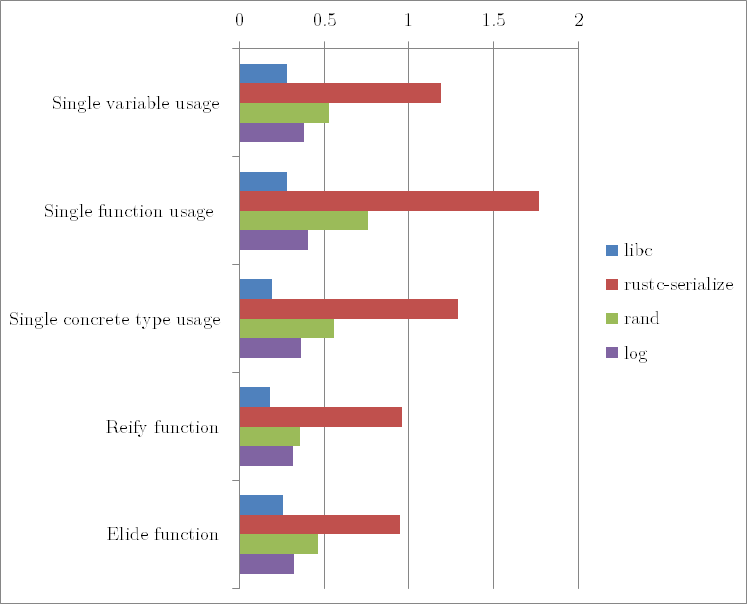
\includegraphics[width=8cm]{refactorings}

\caption{Graph displaying timing in seconds for the different refactorings}
\label{Fig:compareref}
\end{center}
\end{figure}

\subsubsection{Varying the number of refactoring locations or usages}
From `libc', a number of different concrete types were targeted for performing a rename. `libc' was chosen for having a wider variety of occurrence counts specifically with concrete types. Figure \ref{Fig:comparerefs} shows how concrete type renaming appears to scale linearly (as expected from Chapter \ref{C:impl}) with the number of usages. Ideally, this analysis would have been done with other refactorings, but finding a reasonable amount of variation on the number of usages was difficult and searching was mostly manual. All the rename refactorings generally follow similar code paths and so the idea is that they should all scale in the same way (with the same general relationship). In particular, investigating function renaming would have been insightful as they take inherently more time. Although we expect to always scale linearly with the number of usages, the entire compiler is invoked each time instead of running what is actually necessary, like name resolution. As such, improvements can likely be made to the multiplying factor. As for the lifetime refactorings, the selection for the earlier timings did not strongly consider the number of visible `\&' and from observation, the time they took did not generally vary significantly. This is probably because they do not use additional passes of the compiler. Investigating scalability allows us to predict the time required for refactoring larger codebases. Referring back to Fowler, this is important for a tool since taking too long means that a programmer would simply prefer to do the refactoring by hand.

%In particular, Other crates or types of renamings had few examples and only a limited amount of variation.

\begin{figure}[h]
\begin{center}
    \begin{tabular}{ | l | c |}
    \hline
    \textbf{Number of replaced occurrences} & \textbf{Time in seconds} \\ \hline
    1 type usage &  0.1925  \\ \hline
    3 type usages &  0.3821  \\ \hline
    4 type usages &   0.4749  \\ \hline
    6 type usages &   0.6737  \\ \hline
    8 type usages &   0.8739 \\ \hline
    13 type usages  &  1.373 \\ \hline
    29 type usages &  2.960  \\ \hline
    51 type usages &  5.059 \\ \hline
    \end{tabular}
\end{center}

\caption{Timings for varying usage counts of concrete types in libc}
\label{Fig:scaling}
\end{figure}

\begin{figure}[h]
\begin{center}

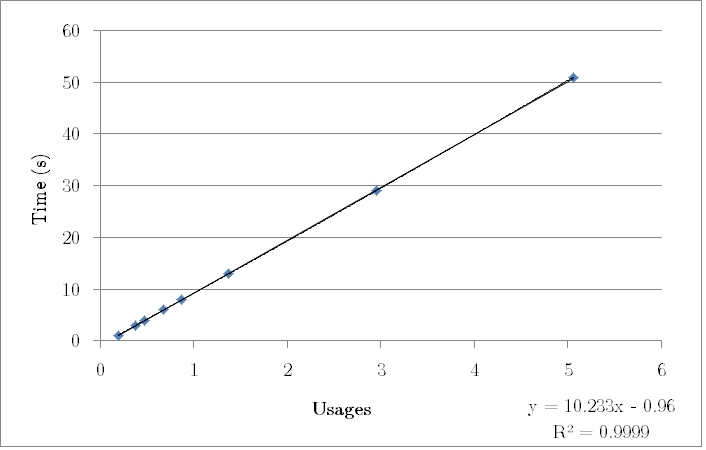
\includegraphics[width=8cm]{scaling}

\caption{Graph displaying results of varying the number of usages}
\label{Fig:comparerefs}
\end{center}
\end{figure}

Rust generally encourages the use of Crates.io and package management to form modular systems. This means that the amount of code implemented by you personally is as minimal as possible, making scalability potentially a non-issue. On the other hand, more modular systems mean more API and shared functions, types etc. While this might not affect performance it affects the overall difficulty of refactoring because once an API is exposed, it is usually not liable to change. Changes across different code-bases are problematic, not just for Rust, but for programmers in general (due to different owners, licenses, etc.).

%\subsection{Other potential methods of evaluation} \label{S:otherstuff}
%%The types of considerations which could have been done are as follows:
%%Design considerations - well, workflow problems
%Comparison to Eclipse or IntelliJ might have provided some useful points of contrast, but the language differences would make many of the comparisons difficult or meaningless. In particular, what is not immediately clear is how much correctness checking these tools actually perform. Eclipse could be investigated by looking at their codebase, but fundamentally Java is quite a different language to Rust with different complexities. There is also Rust specific refactorings here, but a notable point of comparison is definitely inlining. In downloading and installing a recent version of Eclipse, it appears that even the consideration of preventing an inline when the variable appears in a simple assignment was ignored.
%
%A user study may have been another avenue to explore, but this appeared inappropriate for a number of reasons. We could bring in users of Rust, but the language is still in the process of gathering popularity. Finding those with the adequate amount of experience would likely be limited to those working heavily with the language, possibly working on the compiler (when our real target demographic is the casual user of Rust who does not know the inner workings well). There would also be few points of comparison, besides perhaps manual refactoring. A good deal of time was spent just determining what could even be done as part of this tool. Trying to juggle a user evaluation would have detracted from the goal of exploring the actual problems with a specifically Rust, refactoring tool. 

\subsubsection{Limitations in the performance evaluation}

Perhaps the most obvious shortcoming in these tests is the lack of sufficient data points, especially when trying to justify a trend. Finding the current set of examples was already extremely difficult given the size of the crates, made worse by the lack of macro support. Originally, a fifth crate `bitflags' was to be analyzed; however, the entire crate formed a macro expansion, preventing any refactoring. `libc' was almost entirely header declarations, having no `let' bindings, which made it difficult to generate the full set of refactorings. Performing scaling tests on more than just renaming types would have been helpful to prove worst-case linear scaling, especially for renaming functions as it was noticeably slower. But finding any meaningful variation of occurrences was difficult, and having but a few usages was common (as seen by the concentration of points in Figure \ref{Fig:comparerefs}). The relative size of the crates is still quite small and how the tool functions on much larger codebases is still completely unknown. Missing inline definitely limits the amount of useful conclusions that can be draw here. But the fact that few suitable locations for its usage were found questions the usefulness of the refactoring and the associated checks (given how incomplete they are). 
